\documentclass[11pt]{report}

% ----------------------------------------------------
% PACKAGE
% ----------------------------------------------------

\usepackage{graphicx}
\usepackage{amsmath}
\usepackage{amsfonts}
\usepackage{amssymb}
\usepackage{hyperref}
\usepackage[a4paper, portrait, margin=0.5in]{geometry}
\usepackage[italian]{babel}
\usepackage{enumerate}% http://ctan.org/pkg/enumerate

% \usepackage{tcolorbox} % usato per fare le box colorate
% \usepackage{soul} % usato per barrare il testo
% % \usepackage{algorithm} % usato per scrivere algoritmi
% \usepackage{algpseudocode}
% \usepackage{algorithm2e}
% \usepackage{tikz}
\usepackage{circuitikz}
% \usepackage{listings}

% \lstset{
%   language=Python,
%   basicstyle=\ttfamily,
%   keywordstyle=\color{blue},
%   stringstyle=\color{red},
%   commentstyle=\color{green},
%   numbers=left,
%   numberstyle=\tiny\color{gray},
%   breaklines=true,
%   frame=single,
%   captionpos=b,
%   showstringspaces=false,
%   tabsize=2
% }
% \hypersetup{
%     colorlinks=true,
%     linkcolor=black,
%     urlcolor=blue,
% }

\title{Fondamenti di controlli automatici}
\author{Ollari Dmitri}

\begin{document}
    \maketitle

    \tableofcontents
    \chapter{Il controllo attivo di un processo}

Un processo \`e l'evoluzione nel tempo di un sistema.

Con controllo attivo si intende una strategia di controllo del sistema controllato che prevede 
un'azione di controllo che dipende dallo stato del sistema stesso.

\section{Insieme dei Behaviors}

I behaviors sono tutte le possibile coppie causa-effetto associate ad un'sistema.








    \chapter{Modellistica ed equazioni differenziali lineari}

\section{Circuiti elettrici}

\begin{center}
  \begin{tabular}{|l l|}
  \hline
    Resistenza & $v(t) = Ri(t)$ \\
    Induttanza & $v(t) = L\frac{di(t)}{dt} = LDi$ \\
    Capacità & $v(t) = \frac{1}{C}\int_{-\infty}^t i(\tau) \rightarrow Dv_C = \frac{i}{C}$ \\
  \hline
  \end{tabular}
\end{center}

\section{Sistema meccanico}
\begin{center}
  \begin{tabular}{|l l|}
  \hline
    Massa & $MD^2x(t) = f_1(t)-f_2(t)$ \\
    Molla & $f(t) = K(x_1(t) - x_2(t))$ \\
    Ammortizzatore & $f(t) = BD(x_1(t) - x_2(t))$ \\
    \hline
  \end{tabular}
\end{center}



\section{OPAMP}
\begin{figure}[h!]
\centering
  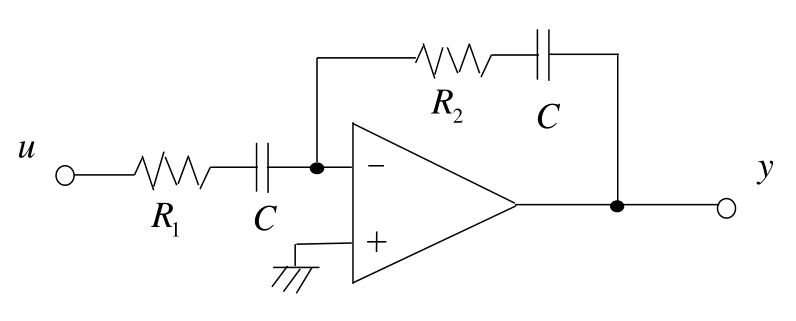
\includegraphics[width=0.4\linewidth]{images/opamp.png}
\end{figure}
Avendo $u$ tensione in ingresso e $y$ tensione in uscita, si ha che:
\begin{align}
  R_1CD_y + y = -R_2CDu - u
\end{align}


\section{Equazioni differenziali lineari}
Generalmente si ha che:

\begin{align}
  \sum_{i=0}^n a_iD^iy = \sum_{i=0}^m b_iD^iu
\end{align}

Dove:
\begin{itemize}
  \item $\rho = |n - m|$ ordine relativo o grado relativo
  \item $y$ è l'uscita
  \item $u$ è l'ingresso
\end{itemize}

    % \chapter{Cenni di analisi complessa}
\section{Poli e zeri}



    \chapter{La trasformata di Laplace}


La trasformata di Laplace \`e un'operazione funionale che si applica ad una funzione $f$ di viariabile 
reale con codominio $R$(o $C$).

\section{Segnale gradino unitario $1(t)$}

\begin{align}
  \mathcal{L}[1(t)] = \frac{1}{s}
\end{align}


\section{Segnale esponenziale $e^{at}$}

\begin{align}
  \mathcal{L}[e^{at}] = \frac{1}{s - a}
\end{align}



\section{Trasformata dell'integrale}

\begin{align}
  \mathcal{L}\Bigg[\int_0^t f(v)dv\Bigg] = \frac{1}{s}F(s)
\end{align}

\section{Trasformata $t^n$}

\begin{align}
  \mathcal{L}[t^n] = \frac{n!}{s^{n+1}}
\end{align}

    % % \chapter{Funzioni inpulsive e insieme di Behaviors}
%
%
% % \section{Cenni di teoria delle funzioni impulsive}
% \section{Derivata generalizzata di una funzione discontinua}
%
%

    \chapter{Funzioni di trasferimento}

\section{Definizioni}
\subsection{Proprio}
Un sistema si dice \textbf{(strettamente) proprio} se la sua funzione di trasferimento
\`e \textbf{(strettamente) propria}.
Quindi con grado relativo $\rho \geq 0$ il sitema \`e proprio, mentre con grado relativo $\rho \geq 1$ il sistema \`e strettamente proprio.


\subsection{Guadagno statico}
Il guadagno statico \`e il valore:
\begin{align}
  K := \frac{y_c}{u_c}
\end{align}

Dove la $y_c$ \`e la risposta del sistema all'ingresso costante $u_c$.


\subsection{Polinomio caratteristico}

Dato il sistema $\sum$ descritto dall'equazione differenziale:
\begin{align}
  \sum_{i=0}^n a_i D^i y = \sum_{i=0}^m b_i D^i u
\end{align}



Il polinomio caratteristico \`e definito come:
\begin{align}
  a(s) = \sum_{i=0}^n a_i s^i
\end{align}


\subsection{Modi del sistema}

I modi sono le funzioni tipiche asociate ai poli del sistema,
se $p$ \`e un polo reale di molteplicit\`a $h$ i suoi modi saranno definito come:

\begin{align}
  e^{pt}, te^{pt}, t^2e^{pt}, \dots, t^{h-1}e^{pt}
\end{align}

Mentre se $p$ \`e un polo complesso coniugato($\sigma + j\omega$) di molteplicit\`a $h$ i suoi modi saranno definito come:

\begin{align}
  e^{\sigma t} \sin(\omega t + \phi_1), te^{\sigma t} \sin(\omega t + \phi_2), \dots, t^{h-1}e^{\sigma t} \sin(\omega t + \phi_h)
\end{align}
Che \`e equivalente a:
\begin{align}
  e^{\sigma t} \sin{\omega t}, e^{\sigma t} \cos{\omega t}, te^{\sigma t} \sin{\omega t}, te^{\sigma t} \cos{\omega t}, \dots, t^{h-1}e^{\sigma t} \sin{\omega t}, t^{h-1}e^{\sigma t} \cos{\omega t}
\end{align}

\subsection{Segnali tipici di ingresso}
\begin{center}
\renewcommand{\arraystretch}{1.5}
  \begin{tabular}{|l|c|c|}
    \hline
    Segnale & $u(t)$ & $U(s)$ \\
    \hline
    Impulso unitario & $\delta(t)$ & $1$ \\
    Gradino unitario & $1(t)$ & $\frac{1}{s}$ \\
    Rampa unitaria & $t(t)$ & $\frac{1}{s^2}$ \\
    Parabola unitaria & $\frac{1}{2}t^2(t)$ & $\frac{1}{s^3}$ \\
    \hline
  \end{tabular}
\end{center}


    \chapter{Sistemi dinamici elementari}

\section{Parametri della risposta al gradino}
\begin{center}
\renewcommand{\arraystretch}{1.5}
  \begin{tabular}{|c|l|}
  \hline
    Simbolo & Descrizione \\
  \hline
    $S$ & Sovraelongazione \\
    $T_r$ & Tempo di ritardo \\
    $T_s$ & Tempo di salita \\
    $T_m$ & Tempo di massima sovraelongazione  \\
    $T_a$ & Tempo di assestamento  \\
  \hline

  \end{tabular}
\end{center}


\section{Sistemi del secondo ordine(senza zeri)}
Per risolvere questo esercizio conviene portare la funzione nella seguente forma:
\begin{align}
  G(s) \frac{\omega_n^2}{s^2+2\delta\omega_ns+\omega_n^2}, \quad G(0)=1
\end{align}

Ovviamente l'equazione differenziale che descrive il sistema è:
\begin{align}
  D^2y + 2\delta\omega_nDy+\omega_n^2y = \omega_n^2u
\end{align}

La pullsaizone naturale è $\omega_n$.

Per determinare la risposta al gradino unitario, si moltiplica la funzione di trasferimento per la trasformata di Laplace del gradino per la funzione di trasferimento,
Dopo di che di ottengono:

\begin{center}
\renewcommand{\arraystretch}{1.5}
  \begin{tabular}{|l|c|}
    \hline
      Pulsazione & $\omega = \omega_n\sqrt{1-\delta^2}$ \\
      Massima sovraelongazione(\%) & $S = 100 \exp\{- \frac{\delta \pi}{\sqrt{1 - \delta^2}}\}$ \\
      Tempo di assestamento & $T_a \approx \frac{3}{\delta \omega_n}$ \\
      Tempo di salita & $T_s \approx \frac{1.8}{\omega_n}$ \\
    \hline
  \end{tabular}
\end{center}


\section{Poli dominanti}
I poli dominanti sono quei poli(normalemnte una coppia) che non sono soggetti a quasi cancellazione 
polo-zero e sono più vicini all'asse immaginario.

    \chapter{Stabilit\`a dei sistemi dinamici}

\section{Stabilit\`a alle perturbazioni}
Bisogna analizzare i punti di equailibrio($G(0)$).


\begin{center}
\renewcommand{\arraystretch}{1.5}
  \begin{tabular}{|l|c|}
    \hline
      stabile & $y_{lib}(t)$ \`e limitata su $[0, +\infty)$ \\
      instabile & $y_{lib}(t)$ non \`e limitata su $[0, +\infty)$ \\
      asintoticamente stabile & $y_{lib}(t) \rightarrow 0$ per $t \rightarrow +\infty$ \\
      semplimente stabile & stabile ma esiste una perturbazione che lo rende instabile \\
      \hline
  \end{tabular}
\end{center}

\section{Poli e stabilitt\`a}


\begin{center}
\renewcommand{\arraystretch}{1.5}
  \begin{tabular}{|l|p{9cm}|}
    \hline
      stabile & $Re(p_i) \leq 0$ ed eventuali poli puramente immaginari semplici \\
      asintoticamente stabile & $Re(p_i) < 0$\\
      semplimente stabile & $Re(p_i) \leq 0$ e i poli puramente immaginari(devono essitere, al massimo uso $s=0$) sono semplici \\
      instabile & $Re(p_i) > 0$ oppure polo puramente immaginario con molteplicit\`a $> 1$  \\
    \hline
  \end{tabular}
\end{center}


\section{Stabilit\`a bounded-input bounded-output(BIBO)}

Un sistema \`e BIBO stabile se ogni ingresso limitato produce un'uscita limitata.

\section{Criterio di Routh-Hurwitz}

Considerando il solito sistema lineare $\sum$ descritto da $\sum_{i=0}^n a_iD^iy = \sum_{i=0}^m b_iD^iu $.

La funzione di trasferimento sar\`a $G(s) = \frac{b(s)}{a(s)}$.


Con il metodo di Routh si pu\`o analizzare la stabilitt\`a di un sistema
senza risolvere l'equazione caratteristica($a(s)=0$) e trovare i poli.


Il polinomio \`e hermitiano solo se i suoi coefficienti sono positivi, per fare questa dimostrazione
si riorre alla tabella di routh.

\subsection{Tabella di Routh}
la tabella di Routh \`e costituita da $n-1$ righe, calcolate a ritroso.

Una volta ordinato il polinomio in ordine decrescente di esponenti:
\begin{align}
  a_n s^n + a_{n-1} s^{n-1} + \dots + a_1 s + a_0 = 0
\end{align}


Si costruiscono le prime due righe della tabella alternando i coefficienti:
\begin{center}
  \begin{tabular}{|c|c|c|c|c|}
    \hline
    n & $a_n$ & $a_{n-2}$ & $a_{n-4}$ & $\dots$ \\
    \hline
    n-1 & $a_{n-1}$ & $a_{n-3}$ & $a_{n-5}$ & $\dots$ \\
    \hline
  \end{tabular}
\end{center}

Si possono calcolare tutte le righe succesive nella seguente maniera:

\begin{center}
  \begin{tabular}{|c|c|c|c|c|}
    \hline
    n & $\gamma_{0,0}$ & $\gamma_{0,1}$ & $\gamma_{0,2}$ & \dots \\
    n-1 & $\gamma_{1,0}$ & $\gamma_{1,1}$ & $\gamma_{1,2}$ & \dots \\
    n-2 & $\gamma_{2,0}$ & $\gamma_{2,1}$ & $\gamma_{2,2}$ & \dots \\
    \dotfill & \dotfill & \dotfill & \dotfill & \dotfill \\
    \hline
  \end{tabular}
\end{center}

Per calcolare $\gamma_{i,j}$ si usa la seguente formula:
\begin{align}
  \gamma_{i,j} = \frac{
    \begin{pmatrix}
      \gamma_{i-2, 0} & \gamma_{i-2, j+1} \\
      \gamma_{i-1, 0} & \gamma_{i-1, j+1}
    \end{pmatrix}
    }{\gamma_{i-1, 0}}
\end{align}

Super TIP: Immagina il calcola da fare come:
\begin{align}
  \frac{
    \begin{pmatrix}
      a & b \\
      c & d
    \end{pmatrix}
  }{c}
  =
  \frac{cb  - ad}{c}
\end{align}

Inoltre consiglio di tracciare una croce immaginaria sulla tabella di routh,
$c \rightarrow b \rightarrow a \rightarrow d \rightarrow c$.




\subsection{Teorema di Routh}
Si esamina la prima colonna della tabella calcolata e si osservgano le variazioni di segno nella prima colonna.

Si determinano il numero di variazioni e permanenze di segno(sommano a $n$).

Assumento di poter completare la tabella, \textbf{ad ogni variazione di segno corrisponde un polo con parte reale positiva}(causa instabilit\`a),
mentre ogni permanenza di segno corrisponde a un polo con parte reale negativa.


\subsection{Singolarit\`a della tabella}

Esistono due casi particolari che occorrono durante il calcolo della tabelle:
\begin{itemize}
  \item Il primo elemento di una riga \`e $0$
  \item Tutti gli elementi di una riga sono $0$
\end{itemize}

Per il primo caso si procede nel seguente modo:
ogni riga non nulla che inizia con $n$ zeri viene sommata con la riga ottenuta
moltiplicandola per $-1^n$ e traslandola verso sinistra di $n$ posizioni.


Se una riga \`e nulla, si procede nel seguente modo:

\begin{enumerate}
  \item Si sceglie come polinomio ausiliario quello della riga immediatamente sopra a quella con gli zeri
  \item Si deriva il polinomio ausiliario
  \item Sostituisco la riga di zeri con i coefficienti del polinomio ausiliario derivato
\end{enumerate}

Quando si far\`a il conteggio delle variazioni e delle permanenze, non ci saranno variazioni nella procedura.




    \chapter{Analisi armonica e diagrammi di Bode}


% \section{Teorema analisi armonica}
% Sia $\sum$ un sistema asintoticamente stabile con funzione di trasferimento $G(s)$ razionale, 
% la risposta forzata 

\section{Guadagno del sistema lineare}

Abbiamo visto 3 tipi di guadagni:
\begin{itemize}
  \item $G(s)$ guadagno dianmico
  \item $G(j\omega)$ risposta in frequenza
  \item $G(0)$ guadagno statico
\end{itemize}


\section{Diagrammi di Bode}
Sono diagrammi cartesiani logaritmici delle risposte armoniche, rappresentano le ampiezze e 
le fasi della risposta in frequenza del sistema. 


\section{Rappresentazione parametri della funzione di trasferimento}

Funzione di trasferimento razionale scritta nella forma standard poli e zeri:
\begin{align}
  G(s) = K_1 \frac{(s-z_1)(s-z_2)\dots(s-z_m)}{(s-p_1)(s-p_2)\dots(s-p_n)}
\end{align}

$K_1$ è il guadagno statico del sistema, $z_i$ sono gli zeri e $p_i$ sono i poli. 

Alcune volte può essere presente un polo nell'origine con uan certa molteplicità $h$:
\begin{align}
  G(s) = K_1 \frac{(s-z_1)(s-z_2)\dots(s-z_m)}{s^h(s-p_1)(s-p_2)\dots(s-p_n)}
\end{align}


\subsection{Modulo e fase}
\begin{align}
  % G(j\omega) = K_1 \frac{(j\omega-z_1)(j\omega-z_2)\dots(j\omega-z_m)}{(j\omega)^h(j\omega-p_1)(j\omega-p_2)\dots(j\omega-p_n)}
  G(j\omega) &= |G(j\omega)|e^{j \arg G(j\omega)} \\
  \alpha &= \ln |G(j\omega)| \\
  \beta &= \arg G(j\omega) \\
  G(j\omega) &= \alpha + j\beta
\end{align}


Di solito si rappresentano le ampiezze in decibel e le fasi in gradi. 
Per calcolare i decibel si usa la seguente formula:
\begin{align}
  db = 20 \log_{10} |G(j\omega)|
\end{align}


Partendo dalla funzione di trasferimento in forma polinomiale:

\begin{align}
  G(j\omega) = K_1 \frac{(j\omega-z_1)(j\omega-z_2)\dots(j\omega-z_m)}{(j\omega)^h(j\omega-p_1)(j\omega-p_2)\dots(j\omega-p_n)}
\end{align}

Per calcolare il modulo si usa la seguente formula:
\begin{align}
  |G(j\omega)| = K_1 \frac{|j\omega-z_1||j\omega-z_2|\dots|j\omega-z_m|}{|j\omega|^h|j\omega-p_1||j\omega-p_2|\dots|j\omega-p_n|}
\end{align}

Dove $|j\omega| = \omega$ e $|j\omega-z_i| = \sqrt{\omega^2 + z_i^2}$

Per la fase si usa la seguente formula:
\begin{align}
  \arg G(j\omega) = \arg K_1 + \arg (j\omega-z_1) + \arg (j\omega-z_2) + \dots + \arg (j\omega-z_m)  \\ 
  - [h\arg (j\omega) + \arg (j\omega-p_1) + \arg (j\omega-p_2) + \dots + \arg (j\omega-p_n)]
\end{align}

Dove $\arg (j\omega) = \frac{\pi}{2}$ e $\arg (j\omega-p_i) = \arctan \frac{\omega}{p_i}$

Quando disegni la fase nei grafici, ricorda che se la $K_1$ è negativa, allora la fase è sfasata di $\pi$(parti da $-\pi$).


\subsection{Parametri di rsiposta armonica}
\begin{center}
  \renewcommand{\arraystretch}{1.5}
  \begin{tabular}{|l|c|}
    \hline
    Pulsa di risonanza & $\omega_r = \arg \max |G(j\omega)|$ \\
    Picco di risonanza & $M_R = \frac{|G(j\omega_r)|}{|G(j0)|}$ \\
    Larghezza di banda & $\Delta \omega = \omega_2 - \omega_1$ \\
    \hline
  \end{tabular}
\end{center}

    \chapter{Diagrammi di Nyquist e sistemi a fase minima}


I diagrammi di Nyquist sono utili per lo studio della stabilit\`a.

I comportamenti pi\`u importanti sono:
\begin{itemize}
  \item $\omega \rightarrow +\infty$
  \item $\omega \rightarrow 0+$ di tipo 0(no poli nell'origine)
  \item $\omega \rightarrow 0+$ di tipo  magiore uguale 1(polo nell'origine e dipende dalla molteplicit\`a)
\end{itemize}


\section{Sistemi a fase minima}
Considerp il sistema lineare e stazionario $\sum$ con funzione di trasferimento $G$ 
e risposta armonica $G(j\omega)$.


$\sum$ \`e a fase minima se il diagramma delle fase $\beta = \arg G(j\omega)$ \`e determinato 
univocamente(modulo $2\pi$) dal diagramma dei moduli $\alpha = |G(j\omega)|$ mediante la formula di Bode.







\section{Formula di}
\begin{align}
  \alpha = \ln |G(j\omega)| \\
  \beta = \arg G(j\omega)
\end{align}





    \chapter{Sistemi retroazionati}

\begin{figure}[h!]
  \centering
  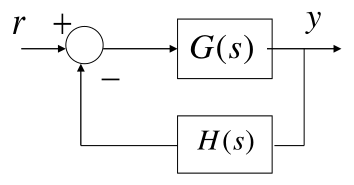
\includegraphics[scale=0.3]{./images/schema_blocchi.png}
\end{figure}

La funzione di trasferimento \`e:

\begin{align}
  f.d.t. = \frac{Y(s)}{X(s)} = \frac{G(s)}{1 + G(s)H(s)}
\end{align}


% \section{Analisi a regime dei sistemi in retroazione}
% \subsection{Gradino}
%
% \begin{align}
%   e_r = \lim_{s \to 0} sE(s) = \frac{r_0}{1 + K}
% \end{align}




    \chapter{Sistemi retroazionati}
Avendo un sistema retrazionato definito da:
\begin{align}
  T(s) = \frac{G(s)}{1+G(s)H(s)}
\end{align}

Il sistema retroazionato \`e ben connesso se:
\begin{align}
  \lim_{|s| \to \infty} G(s)H(s) \neq 0
\end{align}

e la buona connessione \`e necessaria per la stabilit\`a del sistema.



\section{Criterio di Nyquist}
Metodo utile per lo studio della stabilit\`a asintotica.

Il criterio afferma che il sistema retroazionato \`e stabile asintoticamente
se e solo se l'equazione caratteristica $1 + G(s)H(s) = 0$ ha tutte le radici a parte reale 
negativa.

\textbf{Dopo di che il criterio di Nyquist richiede il tracciamento del diagramma di Nyquist di $G(j\omega)H(j\omega)$}.





\subsection{Teorema dell'indice logaritmico}

Se il diagramma di Nyquist ha senso \textbf{orario}:
\begin{align}
  \{\text{numero di giri \textbf{orari} della curva immagine intorno all'origine}\} = n_z - n_p
\end{align}


Mentre se il diagramma di Nyquist ha senso \textbf{antiorario}:

\begin{align}
  \{\text{numero di giri \textbf{antiorari} della curva immagine intorno all'origine}\} = n_z - n_p
\end{align}


Applicando il terorema alla stabilit\`a dei sistemi retroazionati:
\begin{itemize}
  \item $n_z$ \`e il numero di zeri di $1 + G(s)H(s)$ appartenenti a $\mathbb{C}$
  \item $n_p$ \`e il numero di poli di $1 + G(s)H(s)$ appartenenti a $\mathbb{C}$
  \item $\psi$ \`e il numero di giri in senso orario
\end{itemize}

    \chapter{Luogo delle radici}


Eistono due tipologie di luoghi delle radici, diretto e indiretto.

Avendo un guadagno ad anello:
\begin{align}
  L(s) = G(s)H(s) = K_1 \frac{(s-z_1)\dots(s-z_m)}{(s-p_1)\dots(s-p_m)} = K_1G_1(s)
\end{align}

Il luogo delle radici diretto `e descritto da $1 + K_1G_1(s) = 0$ con $K_1$ che varia 
da $0$ a $+\infty$.

Il luogo delle radici inverse ha invece $1 + \frac{1}{K_1G_1(s)} = 0$ con $K_1$ che varia
da $0$ a $-\infty$.


\section{Propriet\`a del luogo delle radici}
\begin{itemize}
  \item Il luogo delle radici ha tanti rami quanti sono i poli di $G_1(s)$.
  \item Ogni ramo parte da un polo di $G_1(s)$ e tende ad un zero di $G_1(s)$.
  \item Il luogo delle radici \`e simmetrico rispetto all'asse reale.
  \item Nel luogo diretto, un punto dell'asse reale fa parte del luogo delle radici se alla sua destra ci sono un numero dispari di poli e zeri.
  \item Nel luogo inverso, un punto dell'asse reale fa parte del luogo delle radici se alla sua destra ci sono un numero pari di poli e zeri.
\end{itemize}




\subsection{Angoli luogo diretto}

\begin{align}
  \{ \text{Angoli partenza da $p_i$} \} = \varphi_i = \pi + \sum_{j = 1}^m \arg(p_i - z_j) - \sum_{j \neq 1} \arg(p_i - p_j) \\
  \{ \text{Angoli arrivo in $z_i$} \} = \psi_i = \pi + \sum_{j = 1}^m \arg(z_i - p_j) - \sum_{j \neq 1} \arg(z_i - z_j)
\end{align}



\subsection{Angoli luogo inverso}
Qui s imetto 0 al posto di $\pi$:

\begin{align}
  \{ \text{Angoli partenza da $p_i$} \} = \varphi_i = \sum_{j = 1}^m \arg(p_i - z_j) - \sum_{j \neq 1} \arg(p_i - p_j) \\
  \{ \text{Angoli arrivo in $z_i$} \} = \psi_i = \sum_{j = 1}^m \arg(z_i - p_j) - \sum_{j \neq 1} \arg(z_i - z_j)
\end{align}


\subsection{Molteplicit\`a}
Se il polo $p_i$ ha molteplicit\`a $h > 1$:
\begin{align}
  h \varphi_i = \pi + \sum_{j = 1}^m \arg(p_i - z_j) - \sum_{j \neq 1} \arg(p_i - p_j) \mod(2\pi) \\
  h \psi_i = \pi + \sum_{j = 1}^m \arg(z_i - p_j) - \sum_{j \neq 1} \arg(z_i - z_j) \mod(2\pi) 
\end{align}



\section{Asintoti del luogo delle radici}
Punto nell'asse reale dove si forma una stella di asintoti(di raggi):
\begin{align}
  \sigma_a = \frac{\sum_{i-1}^n p_i - \sum_{i=1}^M z_i}{n-m}
\end{align}

Gli angoli degli asintoti nel luogo delle radici diretto sono:
\begin{align}
  \vartheta_{a, v} = \frac{(2v+1)\pi}{n-m} \quad v = 0, 1, \dots, n-m-1
\end{align}

\begin{figure}[h!]
  \centering
  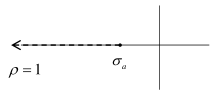
\includegraphics[width=0.15\linewidth]{images/luogo_delle_radici_grado_relativo_1.png}
  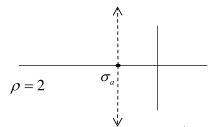
\includegraphics[width=0.15\linewidth]{images/luogo_delle_radici_grado_relativo_2.png}
  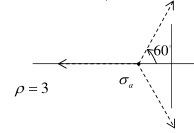
\includegraphics[width=0.15\linewidth]{images/luogo_delle_radici_grado_relativo_3.png}
  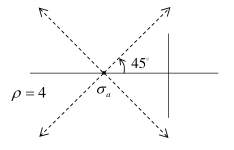
\includegraphics[width=0.15\linewidth]{images/luogo_delle_radici_grado_relativo_4.png}
  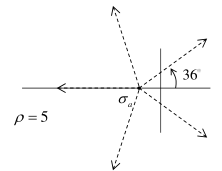
\includegraphics[width=0.15\linewidth]{images/luogo_delle_radici_grado_relativo_5.png}
\end{figure}

Se il luogo dovesse essere inverso:
\begin{align}
  \vartheta_{a, v} = \frac{2v\pi}{n-m} \quad v = 0, 1, \dots, n-m-1
\end{align}


\begin{figure}[h!]
  \centering
  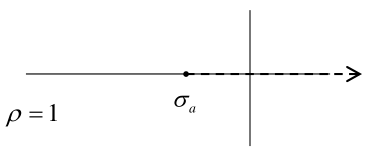
\includegraphics[width=0.15\linewidth]{images/luogo_delle_radici_grado_relativo_1_inverso.png}
  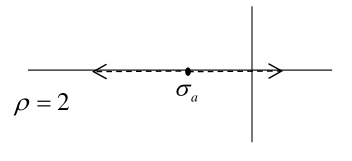
\includegraphics[width=0.15\linewidth]{images/luogo_delle_radici_grado_relativo_2_inverso.png}
  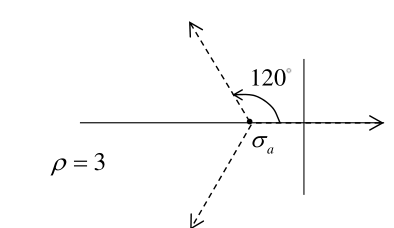
\includegraphics[width=0.15\linewidth]{images/luogo_delle_radici_grado_relativo_3_inverso.png}
  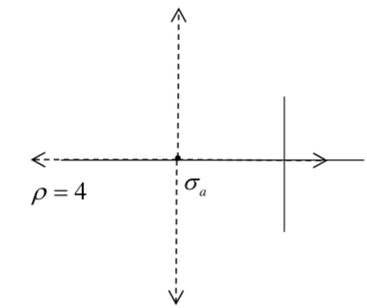
\includegraphics[width=0.15\linewidth]{images/luogo_delle_radici_grado_relativo_4_inverso.png}
  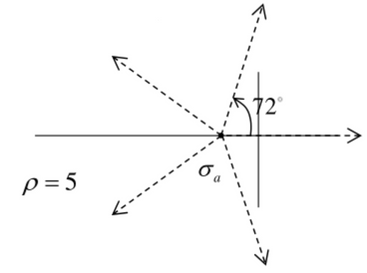
\includegraphics[width=0.15\linewidth]{images/luogo_delle_radici_grado_relativo_5_inverso.png}
\end{figure}





    \chapter{Progetto di un sistema di controllo in retroazione}


\section{Specifiche di progetto}
\begin{enumerate}
  \item Buona connessione(numeratore minore del denominatore)
  \item Stabilit\`a asintotica (radici del denominatore a parte reale negativa)
  \item Prestazioni asintotiche
  \item Prestazioni dinamiche
  \item Robustezza
\end{enumerate}



\section{Regolatori standard}
i regolatori standard si basano sulla combinazione di:
\begin{itemize}
  \item Proporzionale
  \item Integrale
  \item Derivativo
\end{itemize}

La funzione di trasferimento di un controllore proporzionale-integrale-derivativo 
dove $R(s) = (1 + T_d s + \frac{1}{T_i s})$, sviluppando la funzione di trasferimento :
\begin{align}
  R(s) \approx K_p \frac{
    T_d T_i s^2 + T_i s + 1
  }{
    T_i s (1 + \tau s)
  }
\end{align}
  

\section{Rete ritardatrice}
Introduco:
\begin{align}
  C_r(s) = \frac{
    1 + \alpha \tau s
  }{
    1 + \tau s
  }
\end{align}


L'idea alla base della rete ritardatrice \`e quello di attenuare in alta frequenza
il guadagno ad anello, modificando il diagramma polare per ottenere la stabilit\`a.


La rete ritardatrice \`e un filtro passa basso, che attenua le alte frequenze.


Progettiamo $\alpha$ e $\tau$ in modo da assicurare la stabilit\`a asintotica
con un buon margine di ampiezza e fase.

\textbf{Con la rete ritardatrice il guadagno ad anello rimane elevato alle basse frequenze(buone prestazioni statiche)
ma riduce la banda passante(buone prestazioni dinamiche).}

\section{Rete anticipatrice}
\begin{align}
  C_a(s) = \frac{
    1 + \tau s
  }{
    1 + \alpha \tau s
  }
\end{align}



La rete anticipatrice ha diverse caratteristiche:
\begin{itemize}
  \item mantenimento delle prestazioni statiche
  \item stabilizzazione e allargamento banda passante del guadagno ad anello
  \item aumento del grado di stabilit\`a $G_s$
  \item diminuzione del tempo di assestamento $T_a$
  \item miglior capacit\`a di inseguiemento del segnale
\end{itemize}

Lo svantaggio \`e che la rete anticipatrice introduce rumore,
infatti $\alpha$ non pu\`o essere troppo piccolo.

% \section{Sintesi in frequenza}
%
% Avendo una rete anticipatrice:
% \begin{align}
%   C_a(s) = \frac{
%     1 + \tau s
%   }{
%     1 + \alpha \tau s
%   }
% \end{align}
% La converto in frequenza:
% \begin{align}
%   C_a(j \omega) = \frac{
%     1 + j \omega \tau
%   }{
%     1 + j \alpha \omega \tau
%   }
% \end{align}
%
% Posso calcolare modulo e fase:
%
% \begin{align}
%   M &= \frac{
%     \sqrt{1 + \omega^2 \tau^2}
%   }{
%     \sqrt{1 + \alpha^2 \omega^2 \tau^2}
%   }\\
%   \varphi &= \arctan(\omega \tau) - \arctan(\alpha \omega \tau)
% \end{align}
%
% Per effettuare l'inverso, avendo modulo e fase:
%
% \begin{align}
%   \alpha &= \frac{
%     M \cos \varphi - 1
%   }{
%     M (M - \cos \varphi)
%   } \\
%   \tau \omega &= \frac{
%     M - \cos \varphi
%   }{
%     \sin \varphi
%   }
% \end{align}
%
% \subsection{Rete anticipatrice e imposizione del margine di fase}
%
% Scegliere $\omega_0$ affinch\`e:
% \begin{align}
%   \varphi_0 = M_F - \arg L (j \omega_0) - \pi
% \end{align}
%
% valga:
% \begin{align}
%   \cos \varphi_0 > | L(j \omega_0) |
% \end{align}
%
% dopo aver definito:
% \begin{align}
%   M &= \frac{
%     1
%   }{
%     | L(j \omega_0) |
%   } \\
%   \varphi &= \varphi_0  \\
%   \tau &= \frac{
%     M - \cos \varphi
%   }{
%     \omega_0 \sin \varphi
%   } \\
%   \alpha &= \frac{
%     M \cos \varphi - 1
%   }{
%     M (M - \cos \varphi)
%   }
% \end{align}
%
% \begin{align}
%   M_F(\omega_0) = \pi + \arg L(j \omega_0) + \arccos | L(j\omega_0) |
% \end{align}
%
%
% \subsection{Rete ritardatrice e imposizione del margine di fase}
%
% Si sceglie $\omega_0$ affinch\`e:
% \begin{align}
%   \varphi_0 = \arg L(j \omega_0) + \pi - M_F
% \end{align}
%
% con $\varphi_0 > \frac{1}{|L(j\omega_0)|}$
%
% Segue che:
% \begin{align}
%   M = | L(j\omega_0) | \\
%   \varphi = \varphi_0 \\
%   \tau = \frac{
%     M - \cos \varphi
%   }{
%     \omega_0 \sin \varphi
%   } \\
%   \alpha = \frac{
%     M \cos \varphi - 1
%   }{
%     M (M - \cos \varphi)
%   }
% \end{align}
%
%
% \subsection{Rete anticipatrice e imposizione del margine di ampiezza}
%
% PAGINA 37 -> 41





    \chapter{Sistemi di controllo per la regolazione}

Si ha un sistema $P(s)$ e vogliamo determinare un controllore $C(s)$ per il quale si abbia
stabilità asintotica e un errore a regime nullo in risposta al gradino del segnale di riferimento.



Assumo $P(s) = \frac{b(s)}{a(s)}$ con $b(s)$ e $a(s)$ coprimi fra loro,

il problema di regolazione asintotica ha soluzione solo se $P(0) = \neq 0$,
quindi non devono esistere zeri nell'origine.


Possiamo progettare un controllore di ordine $n-1$ affinch\`e i poli 
della retroazione abbiano parte reale negativa e diversi dalle radici di 
$a(s)$ e $b(s)$.





    % \chapter{Regolatori PID}
%
% Ricordo che la funzione di trasferimento di un regolatore PID è:
%
% \begin{align}
% R(s) = K_p \Bigg( 1 + T_d s + \frac{1}{T_i s} \Bigg)
% \end{align}
%
% Riscrivo $R(s)$ per ottenere $\omega_n$ e $\delta$:
%
% \begin{align}
%   R(s) &= K_p \Bigg( 1 + \frac{T_d}{T_i} \frac{1}{s} + \frac{1}{T_i s} \Bigg) \\
%   &= \frac{K_p}{T_i} \frac{
%     T_d T_i s^2 + T_i s + 1
%   }{
%     s
%   } \\
%   &= \frac{K_p}{T_i} \frac{
%     1 + 2 \delta \frac{s}{\omega_n} + \frac{s^2}{\omega_n^2}
%   }{
%     s
%   } \\
% \end{align}
%
% Quindi $\omega_n$ e $\delta$ sono:
% \begin{align}
%   \omega_n &= \frac{1}{\sqrt{T_d T_i}} \\
%   \delta &= \frac{1}{2} \sqrt{\frac{T_i}{T_d}}
% \end{align}
%
% Passando alle frequenze, si ha che:
% \begin{align}
%   R(j\omega) = \frac{K_p}{T_i} \frac{2\delta}{\omega_n} = K_p
% \end{align}
%
% Mentre se la frequenza \`e $\omega_n$:
%
% \begin{align}
%   R(j\omega_n) = \frac{K_p}{T_i} \frac{1}{\omega_n^2} = \frac{K_p}{T_d} = K_p
% \end{align}
%
%
% \section{Implementazione regolatori PID}
%

    % \chapter{Controllo dei sistemi con ritardo}




    \chapter{Introduzione al controllo digitale}

\section{Convertitore A/D}

Convertitore che campiona il segnale analogico in digitale con periodo $T$.

\begin{align}
  x(t) \rightarrow x(kT), \quad k \in \mathbb{Z}
\end{align}



Come Shennon ci ricorda dalle superiori, se la massima frequenza di un segnale
che si vuole campionare \`e $f_{max}$, allora la frequenza di campionamento
dovr\`a essere \textbf{almeno} $2f_{max}$.

La pulsazione di campionamento \`e $\Omega = \frac{2\pi}{T}$.

\section{Trasformata $\mathcal{Z}$}

Sia $x: \mathcal{Z} \rightarrow \mathbb{R}$ o ($\mathbb{C}$) un segnale
a tempo discreto, la trasforamta $\mathcal{Z}$ di $x(k)$ \`e definita come:
\begin{align}
  \mathcal{Z}[x] = \mathcal{Z}[x(k)] = \sum_{k=0}^{+\infty} x(k) z^{-k}
\end{align}

Dove la variabile $z$ \`e una variabile complessa.


Introduco la regione di convergenza (ROC): data la sequanza $x(k)$, la ROC 
di $X(s) = \mathcal{Z}[x(k)]$ \`e definita come:
\begin{align}
  \{ z \in \mathbb{C} : | \sum_{k=0}^\infty x(k)z^{-k} | < \infty \}
\end{align}






    \chapter{Propriet\`a della trasformata $\mathcal{Z}$}



\section{Trasformata di un segnale ritardato di $n$ passi}
\begin{align}
  \mathcal{Z}[x(k-n)] = z^{-n} \mathcal{Z}[x(k)] + \sum_{k=0}^{n-1} x(k-n) z^{-k}
\end{align}



\section{Segnale anticipato di $n$ passi}

\begin{align}
  \mathcal{Z}[x(k+n)] = z^{n} \mathcal{Z}[x(k)] - \sum_{i=0}^{n-1} x(i)z^{n-i}
\end{align}



\section{Teoriema del valore iniziale}
\begin{enumerate}
  \item Se $X(z)$ non ha poli nell'origine $|z| \geq 1$, vuol dire che i poli sono 
  concentrati nel cerchio unitario
  \item Se $X(z)$ non ha poli nell'origine $|z| \geq 1$ eccetto un polo semplice in 
  $z=1$ allora $x(k)$ converge all'infinito
  \item Se $X(z)$ ha un polo multiplo in $z=1$ allora non converge 
  \item Se $X(z)$ ha un polo nella regione $|z| \geq 1, z \neq 1$ allora non converge
\end{enumerate}

\section{Trasformata $\mathcal{Z}$ di $a^k x(k)$}
\begin{align}
  \mathcal{Z}[a^k x(k)] = X(\frac{z}{a})
\end{align}

\section{Convoluzione a tempo discreto}
\begin{align}
  (x * y)(k) = x(k) * y(k) = \sum_{i=-\infty}^{+\infty} x(k-1)y(i)
\end{align}

La trasofrmata $\mathcal{Z}$ della convoluzione \`e:
\begin{align}
  \mathcal{Z}[x(k) * y(k)] = X(z)Y(z)
\end{align}

\section{Derivata della trasformata $\mathcal{Z}$}

\begin{align}
  -z \frac{d}{dz} X(z) = \mathcal{Z}[k x(k)]
\end{align}

    \chapter{Antitrasformata $\mathcal{Z}$}




\end{document}

